\chapteropen{Chapter 1: Software engineering and the SDLC}{chapter-1}
\markboth{Ch. 1 | SDLC}{}


\begin{studycolumns}
\vspace{0pt}
\begin{eli5box}
Building software is like building a playground. First ask who needs it and what they need; then draw plans, choose the structure, build it, check it and keep repairing it. The drawings and checklists are work products. A process explains how the team revisits those activities, not merely a row of boxes.
\end{eli5box}
\textbf{Answer check:} Trace the case from requirement to model, design and test. Process models arrange activities; architectures arrange components; patterns solve recurring design problems. Test design starts before execution.


\needspace{289pt}
\par\smallskip\noindent\begin{minipage}{\linewidth}\centering
\begin{minipage}[t]{0.488\linewidth}\centering\scriptsize\textbf{1}\par\smallskip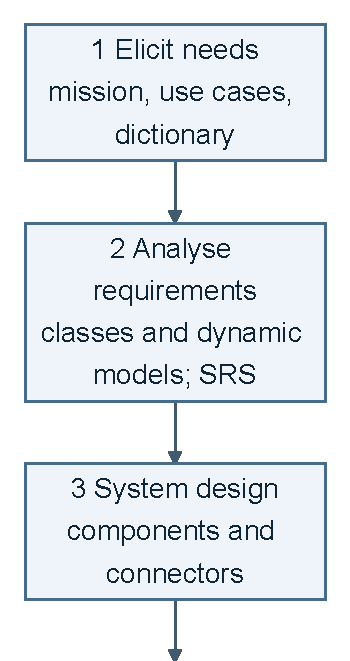
\includegraphics[width=103.04pt]{images/fig-001-compact-1.pdf}\end{minipage}\hfill
\begin{minipage}[t]{0.488\linewidth}\centering\scriptsize\textbf{2}\par\smallskip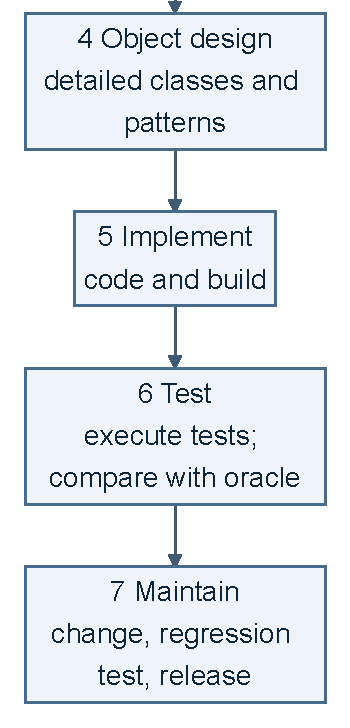
\includegraphics[width=103.04pt]{images/fig-001-compact-2.pdf}\end{minipage}
\captionof{figure}{1. The spine of the course: SDLC \ensuremath{\rightarrow} artefacts --- follow numbered panels; crossing arrows continue.}\end{minipage}\par\smallskip


\needspace{4\baselineskip}
\subsection*{Milestones and work products (L1 work-product table)}
\sectionlabel{h-milestones-and-work-products-l1-work-product-table}

\begin{referenceentries}
\textit{\textbf{Phase} / \textbf{Work products /\allowbreak{} milestones}}\par\smallskip
\noindent \textbf{Requirements specification}: SRS, prototype, requirements review\par
\noindent \textbf{Design}: Software Design Document, Interface Design Document, models, \textbf{test cases}; preliminary \& final design reviews\par
\noindent \textbf{Implementation}: Source code, system build, technical documentation, user manual\par
\noindent \textbf{Testing}: Test execution, test report, user acceptance test\par
\noindent \textbf{Maintenance}: Change request, bug report, patch release, upgrade\par
\end{referenceentries}
\needspace{4\baselineskip}
\subsection*{Definition to memorise}
\sectionlabel{h-definition-to-memorise}

\begin{quote}\small\color{navy}
\textbf{Software engineering} is \emph{the production of maintainable, fault-free software that meets the user's requirements and is delivered on time and within budget.}

\end{quote}


\needspace{4\baselineskip}
\subsection*{The four process activities (also the exam-safe summary)}
\sectionlabel{h-the-four-process-activities-also-the-exam-safe-summary}
\textbf{Specification} (what it should do) \ensuremath{\rightarrow} \textbf{Design \& implementation} (organisation + code) \ensuremath{\rightarrow} \textbf{Validation} (does it do what the customer wants) \ensuremath{\rightarrow} \textbf{Evolution} (change in response to need).


\begin{quote}\small\color{navy}
\textbf{Trap:} process models arrange SDLC activities; architectures arrange components/connectors; design patterns solve recurring object-collaboration problems.

\end{quote}
\end{studycolumns}

\subsection*{Requirement \ensuremath{\rightarrow} analysis \ensuremath{\rightarrow} design traceability chain}
\sectionlabel{h-requirement--analysis--design-traceability-chain}


\par\smallskip\noindent\begin{minipage}{\linewidth}\centering
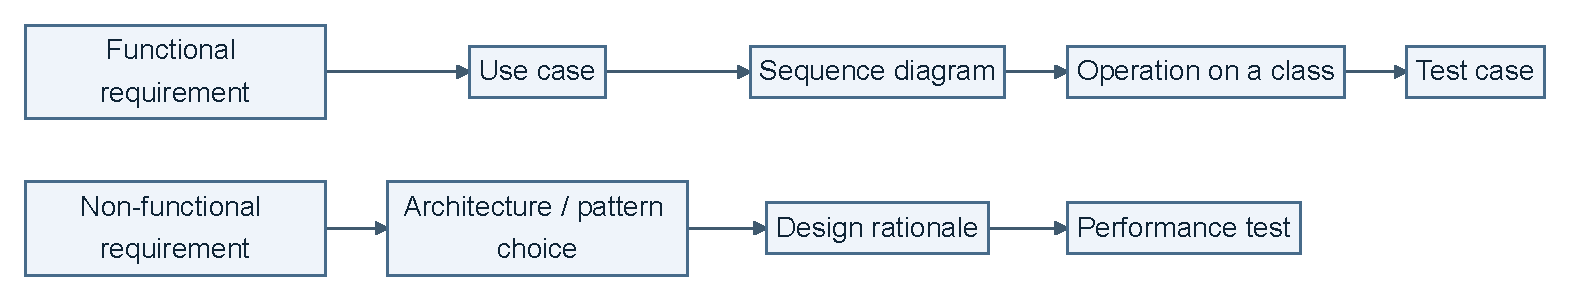
\includegraphics[width=462.30pt]{images/fig-002.pdf}
\captionof{figure}{Requirement \ensuremath{\rightarrow} analysis \ensuremath{\rightarrow} design traceability chain}\end{minipage}\par\smallskip



